\chapter{Implementation approaches} \label{chapter:implementations}

There are several different ways in which we can approach solving the campus navigation problem. Therefore, we would like to explore several different approaches for implementing this functionality, to compare them and decide on the best solution.

\section{Alternatives considered} \label{3:alternatives_considered}

    This section describes the variables explored when researching campus navigation solutions. In order to decide on the best alternative, we compare different approaches for things like technologies, algorithms, positioning strategies and map representations.

    \subsection{Integration with existing tools}
        
        As we've seen in chapter \ref{chapter:sota}, section \ref{2:existing_tools}, there are already some existing solutions for offering \acrshort{upb} students university-related information. We would like to have a tight integration with these tools, both to avoid duplicating efforts, as well as to not overwhelm students even further with more tools that achieve the same goal.
        
        Given that \textbf{\gls{app}} aims to be an information hub, we could potentially integrate the navigation functionality directly within the app as an additional feature. This approach could benefit from the app's involved open-source community, ensuring that the functionality will be extended and maintained over time. Alternatively, we could implement navigation as a separate app, and allow it to be opened from \textbf{\gls{app}} via intents\footnote{\url{https://developer.android.com/guide/components/intents-filters}} or URLs \footnote{\url{https://developer.apple.com/documentation/uikit/interprocess_communication}}. However, even with this second approach, it would be beneficial to make use of the same \gls{firebase} endpoint in order to benefit from the data stored in the app (see the features described in \ref{1:functionalities_core}). Furthermore, \gls{firebase} offers a Dynamic Links\footnote{\url{https://firebase.google.com/docs/dynamic-links}} feature, which can simplify linking between different apps.
        
        The goals of the \textbf{UPB Campus} app are the most closely related to the goals of this study. Therefore, it comes to reason to collaborate and attempt to create a consistent user experience. In terms of integration, the easiest approach here would be again to create a separate app, and allow it to open or be opened from the \textbf{UPB Campus} app. Alternatively, there is a possibility to integrate our features directly within this app as well. However, the process would be more difficult, given that \textbf{UPB Campus} is closed-source and owned by the university.
        
        Finally, we can use the 3D models created through the \textbf{3DUPB} program for navigation. However, simplifiying the models may be needed for smooth operation on mobile devices.
    
    \subsection{Technologies \& APIs} \label{3:technologies_and_apis}
        
        As described in chapter \ref{chapter:sota}, existing solutions are leveraging many different APIs and technologies to achieve various navigation-related functionalities. To this end, we would like to explore several different architectures and approaches in order to pick the best fit.
        
        ~
        
        Firstly, we can look at the existing technologies that we would like to integrate with. Both \textbf{\gls{app}} and \textbf{UPB Campus} share a very similar technology stack, tightly-knit in the Google development ecosystem. They are cross-platform applications built using \gls{flutter}, an open-source UI software development kit developed by Google. \gls{flutter} allows having a shared code-base (written in the Dart programming language) for an application that can be compiled for multiple platforms, the most notable of which being Android and iOS. Furthermore, both apps use the \gls{firebase} platform for the back-end, leveraging services such as a non-relational database (Firestore), notifications, and cloud functions.
        
        ~
        
        One common denominator between the implementations described below is the chosen \textbf{game engine}: \textbf{\gls{unity}}. While our project is not a game, it requires 2D and 3D rendering capabilities that mobile frameworks on their own cannot easily perform, therefore we had to look into choosing an appropriate game engine. The two main picks were \gls{unreal} and \gls{unity}, the two most popular cross-platform game engines. We chose \gls{unity} for multiple reasons. First, we want to have both a 3D and 2D version of the map, and \gls{unity} offers specialized tools for 2D game development. Second, \gls{unity} offers better support for AR functionalities, which we would like to explore for the purpose of indoor navigation. Third, \gls{unity} is compatible with \gls{flutter} through the \mintinline{latex}{flutter_unity_widget}\footnote{\url{https://pub.dev/packages/flutter_unity_widget}}, and while the recommended game engine for \gls{flutter} is Flame\footnote{\url{https://github.com/flame-engine/flame}}, it is a minimalistic engine and not as powerful and versatile as \gls{unity}.
        
        It is worth noting here that the primary programming language used with \gls{unity} is C\#, which comes with all the features of a modern programming language and the powerful built-in Visual Studio support.
        
        ~
        
        Unity also offers a platform-agnostic AR platform called \textbf{ARFoundation}. It is built on top of platforms like ARCore and ARKit (see section \ref{2:ar_technologies}). Furthermore, it leverages common functionalities through a shared API (similar to how Flutter leverages native iOS/Android development components through a single codebase). While it also supports other frameworks (Magic Leap, HoloLens XR Plugins), we are interested in the ARCore/ARKit feature set\footnote{\url{https://docs.unity3d.com/Packages/com.unity.xr.arfoundation@4.1/manual/index.html}} (table \ref{3:tab:unity_ar_support})..
        
        \begin{table}[th]\small\linespread{1}
            \caption{Unity feature support for ARCore/ARKit, according to documentation}
            \label{3:tab:unity_ar_support}
            \centering
            %\resizebox{\textwidth}{!}{
            \begin{tabular}{|l|c|c|}
                \cline{2-3}
                \multicolumn{1}{c|}{} & \textbf{ARCore} & \textbf{ARKit} \\ \hline
                \textbf{Device tracking} & \faCheck & \faCheck \\
                \hline
                \textbf{Plane tracking} & \faCheck & \faCheck \\
                \hline
                \textbf{Point clouds} & \faCheck & \faCheck \\
                \hline
                \textbf{Anchors} & \faCheck & \faCheck \\
                \hline
                \textbf{Light estimation} & \faCheck & \faCheck \\
                \hline
                \textbf{Environment probes} & \faCheck & \faCheck \\
                %\hline
                %\textbf{Face tracking} & \faCheck & \faCheck \\
                %\hline
                %\textbf{2D Image tracking} & \faCheck & \faCheck \\
                \hline
                \textbf{3D Object tracking} & \faClose & \faCheck \\
                \hline
                \textbf{Meshing} & \faClose & \faCheck \\
                \hline
                \textbf{2D \& 3D body tracking} & \faClose & \faCheck \\
                \hline
                \textbf{Collaborative participants} & \faClose & \faCheck \\
                \hline
                \textbf{Human segmentation} & \faClose & \faCheck \\
                \hline
                \textbf{Raycast} & \faCheck & \faCheck \\
                \hline
                \textbf{Pass-through video} & \faCheck & \faCheck \\
                \hline
                \textbf{Session management} & \faCheck & \faCheck \\
                \hline
                \textbf{Occlusion} & \faCheck & \faCheck \\
                \hline
            \end{tabular}
            %}
        \end{table}
        
        Moreover, as we have seen in section \ref{2:maps_apis} of chapter \ref{chapter:sota}, there are several maps APIs that could be used as a source of truth for our functionality, the most notable of which being the Google Maps Platform\footnote{\url{https://developers.google.com/maps}}.

    \newpage
    
    \subsection{Pathfinding strategy}
    
        Pathfinding has been an important topic in multiple domains such as robotics, video games and, of course, navigation. Depending on the environment that a path needs to be found in, many different strategies can be implemented, from traditional strategies such as A* and Dijkstra \cite{graham2003pathfinding}, to neural networks optimized for real-time pathfinding \cite{graham2004neural}. At its core, a pathfinding algorithm has two main requirements: the ability to travel to a specified goal in a given space, and the ability to avoid static and dynamic obstacles along the way. For our use case (campus navigation), dynamic obstacles are not a concern, therefore sophisticated real-time pathfinding algorithms are not necessary. We are only interested in taking the known path on an alley/road as well as indoors, where the obstacles to be avoided are only static (e.g. walls).
    
        Since pathfinding is an important challenge in video games, there are several pathfinding solutions for \gls{unity} available, including the built-in NavMesh Pathfinding. While many developers implement their own solutions or use the built-in one, there are several packages on the \gls{unity} Asset Store which promise pathfinding solutions for game developers. Some of these are specialized (e.g. A* Tile Pathfinding, PolyNav - 2D Pathfinding etc.), while others are more generic (e.g. A* Pathfinding Project, Open World PathFinding System). Among these, by far the most popular (and in the top most popular assets overall) is the A* Pathfinding Project, which offers both a full-fledged “Pro” version as well as a free option with fewer features. Table \ref{3:tab:pathfinding} shows a comparison of the two versions and the built-in \gls{unity} Pathfinding, based on data from the A* Pathfinding Project's website\footnote{\url{https://arongranberg.com/astar/}}.
        
        \begin{table}[th]\small\linespread{1}
            \caption{Pathfinding solutions comparison}
            \label{3:tab:pathfinding}
            \centering
            \resizebox{\textwidth}{!}{
            \begin{tabular}{|l|c|c|c|}
                \cline{2-4}
                \multicolumn{1}{c|}{} & \textbf{A* Pathfinding} & \textbf{A* Pathfinding} & \textbf{Unity NavMesh} \\
                \multicolumn{1}{c|}{} & \textbf{Project Pro} & \textbf{Project Free} & \textbf{Pathfinding} \\ \hline
                \textbf{Cost} & \$100 & free & free \\ \hline
                \textbf{Source code included} & \faCheck & \faCheck & \faClose \\ \hline
                \textbf{Access to pathfinding data} & \faCheck & \faCheck & \faClose \\ \hline
                \textbf{Multiple graphs} & \faCheck & \faCheck & \faCheck \\ \hline
                \textbf{Node penalties} & \faCheck & \faCheck & \faClose \\ \hline
                \textbf{Automatic navmesh generation} & \faCheck & \faClose & \faCheck \\ \hline
                \textbf{In-game graph recalculation} & \faCheck & \faCheck & \faCheck \\ \hline
                \textbf{Built-in editor support} & \faClose & \faClose & \faCheck \\ \hline
            \end{tabular}
            }
        \end{table}
        
        Given that the basic functionalities we are interested in are offered by both the built in solution as well as this package, and that the built in solution has official support and more available resources, we believe that the Unity Navmesh Pathfinder is the best solution for our project.
    
    \subsection{Positioning strategy}
    
        As stated previously, innovation in the field of indoor positioning is not part of the goals of this paper. However, we can explore existing state-of-the-art approaches in order to provide students with a fleshed-out user experience. We would like to visually display the user's current location on the map, even if only approximated.
        
        ~
        
        The most critical position we need is the user's starting location. Once we have that as well as the destination, we can display the navigation path. The user can then use it to navigate on their own, without requiring their permanently updated location (although it would be a quality-of-life improvement).
        
        The most basic approach would be to simply prompt the user to pinpoint their own location on the map. This could be done through the user pressing on a specific point on the in-app map. However, this method comes with significant drawbacks. Firstly, it would require the user to actually know where they are -- which, given that they need a map, is very likely not the case. Secondly, even if the user knows their current location, selecting the right spot on the map may be finicky.
        
        A potentially more reliable way for the user to select their own current position would be for them to enter a string signifying a \acrlong{poi}. We can then associate the given \acrshort{poi} with the corresponding map coordinates, and place the user avatar accordingly.
        
        ~
        
        Both approaches outlined above can be further improved by using \gls{gps} technology. Although we've already established in chapter \ref{chapter:sota} that \gls{gps} is not enough for indoor positioning, it should still provide a location accurate to approximately 5-10 meters. We can use this location to immediately estimate the user's position on the map (that the user can then further correct), or to suggest nearby \acrshort{poi}s. Subsequently, the overhead for using the \gls{gps} location for indoor positioning is effectively zero, considering we would  use it for outdoor navigation either way.
        
        ~
        
        For classic map-based navigation, an approximate position may be enough, given the approaches outlined above. However, when using AR, the accuracy of the initial position may make or break the entire navigation experience. We've seen in section \ref{2:ar_indoor_positioning} that, while ARKit/ARCore can be used for the actual AR navigation, the initial positioning can still be tricky if we can only use location markers on iOS (see section \ref{2:visual_positioning_system}).  Since location markers and similar solutions require extensive mapping beforehand (see section  \ref{2:other_ar_approaches}), we could potentially benefit from a \acrshort{slam} (\acrlong{slam}) solution. This involves real-time generation of a map while simultaneously tracking the agent’s position within it. This can enable us to create an indoor positioning system that doesn’t require preparation beforehand, or, at the very least, requires minimal preparation as opposed to the other techniques described.
        
        ARCore uses \acrshort{slam} out of the box, so for our specific use case, a good solution would be to use \acrshort{slam} to track the user’s location on a known 2D map. But while ARCore can track the user’s movement compared to a starting point, we still need to map this (again, critical) starting point to a known coordinate on the map. Here, we can take advantage of the fact that the user needs to open their camera for AR navigation. Therefore, one way to pinpoint the location could be by using aptly-placed QR codes at specific points in the campus, that users can scan to let the app know where their current location is. This can be especially useful for events taking place in the campus, where a QR code could be placed at the campus entrance.

    \subsection{Map representation}
    
        Aside from the navigation logic itself, an important problem for our project is how to represent the campus map in the app. We can draw it manually, find a way to generate it automatically, or use mixed methods.

        \subsubsection{Source of truth}
        
            The “traditional” way to get the maps would be to use the official floor plan/campus images. However, these are not publicly available, and are generally inconsistent. They can be improved by manually redrawing them to be consistent and making sure they are to scale (and match the corresponding GPS coordinates). This does, however, require significant manual work if no other data is provided, as it would essentially require doing measurements by hand in the campus. Implementation \#4 (see section \ref{3:impl4}) uses drawn 2D maps as the source of truth. Similarly, Implementation \#2 (see section \ref{3:impl3}) also uses static, hand-crafted data in the form of campus building models from 3DUPB (see section \ref{2:existing_tools}). 
            
            Ideally, we’d also like to use some accurate cartographic data to map the GPS coordinates to the points of interest. Implementation \#1 (see section \ref{3:impl1}) uses Google Maps as the source of truth by leveraging the Google Maps SDK for \gls{unity}\footnote{https://developers.google.com/maps/documentation/gaming/overview\_musk}.
            
            Implementation \#3 (see section \ref{3:impl3}) explores another method, which is to use MapsModelsImporter\footnote{https://github.com/eliemichel/MapsModelsImporter}, a Blender add-on for importing 3D models from Google Maps. This creates maps with a greater level of details for smaller areas, that we can then combine to create a full map of the campus.
            
        \subsubsection{In-app representation}
        
            Now that we discussed where the mapping data could come from, we need to describe the concrete representation of this data in the app. There are two important characteristics of our maps: dimensionality (3D vs 2D maps, see figure \ref{3:fig:3dvs2dmaps}) and level of detail. 3D maps can provide more information compared to 2D maps, but can also be more difficult to follow for some users. 2D maps can have other advantages as well, such as making it easier for users to estimate distances\cite{harrower2020to3d}.
            
            \begin{figure}[ht]
                \centering
                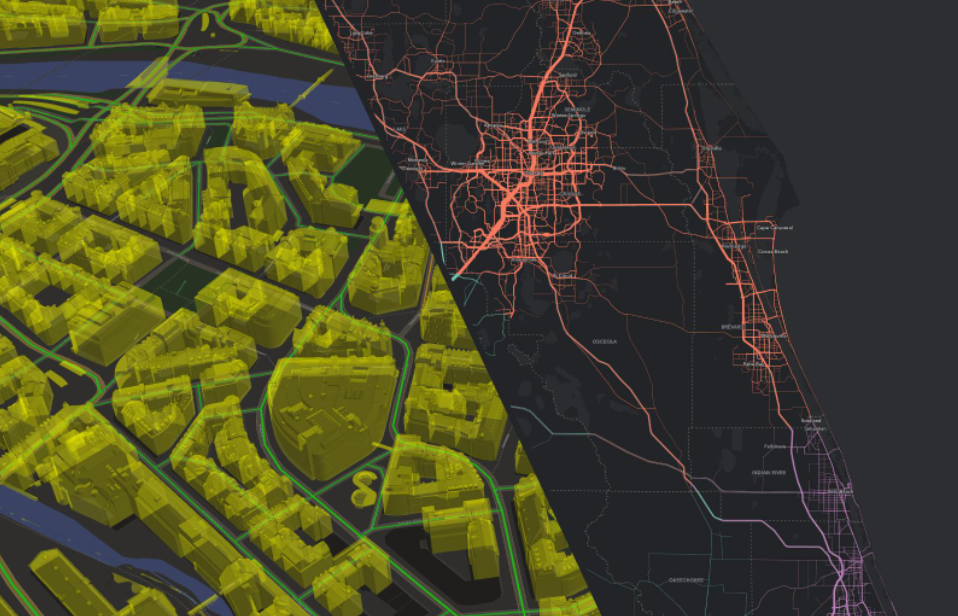
\includegraphics[width=\textwidth]{figures/3dvs2dmap.png}
                \caption{3D vs 2D maps}
                \label{3:fig:3dvs2dmaps}
            \end{figure}
            
            In terms of level of detail, the more components in a map, the more resources will be needed to render it, which can be particularly taxing in the context of a mobile application. From an aesthetic perspective, digital design has been shifting more and more towards a “less is more” approach, and what is called a “flat design”. Therefore, maps with fewer details not only have the advantage of being easier to render (and thus speeding up an app), but they may also be perceived as “cleaner”.
            
            Ultimately, there is no ideal solution, and even Google acknowledges that and simply lets the user choose their own preference, as seen in figure \ref{3:fig:googlemaps_types}.
            
            \begin{figure}[ht]
                \centering
                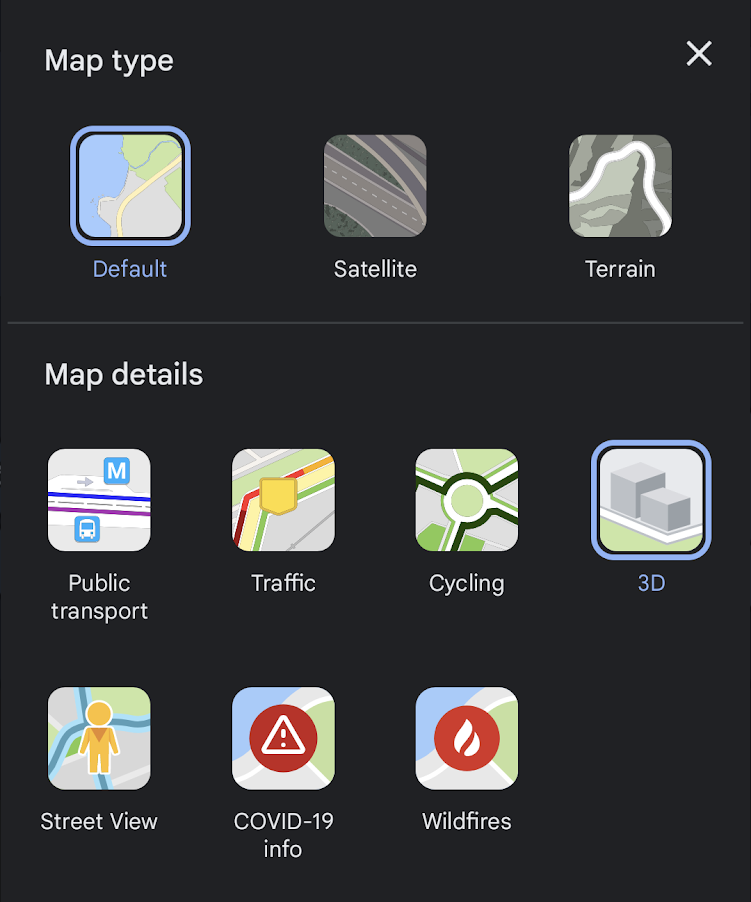
\includegraphics[width=0.6\textwidth]{figures/googlemaps_types.png}
                \caption{Google Maps map options}
                \label{3:fig:googlemaps_types}
            \end{figure}


\section{Implementations overview} \label{3:implementations_overview}

    In order to explore the different variables listed above in various combinations, we implemented multiple proofs of concept as separate Unity scenes and modules. These can be used separately or together as part of a full-fledged navigation application.

    \subsection{Impl. \#1: \gls{flutter} \& Google Maps SDK for \gls{unity}} \label{3:impl1}
    
        For the first implementation, we experimented with direct \gls{flutter} integration in \gls{app}. For the source of truth, we used Google Maps SDK for Unity\footnote{\url{https://developers.google.com/maps/documentation/gaming/overview_musk}} to generate a low-detail 3D representation of the university campus.
    
        \subsubsection{Campus map generation}
        
            Unity calls into the Google Maps API using an API key to obtain information about buildings and roads in a given area, which we then render appropriately (fig. \ref{3:fig:maps_sdk_for_unity_buildings}). The Maps SDK for Unity generates multiple GameObjects as represented in fig. \ref{3:fig:maps_sdk_for_unity_gameobjects}, with the \mintinline{text}{placeID} in brackets.
            
            \begin{figure}[!ht]
                \centering
                \begin{minipage}[b]{0.49\textwidth}
                    \captionsetup{justification=centering}
                    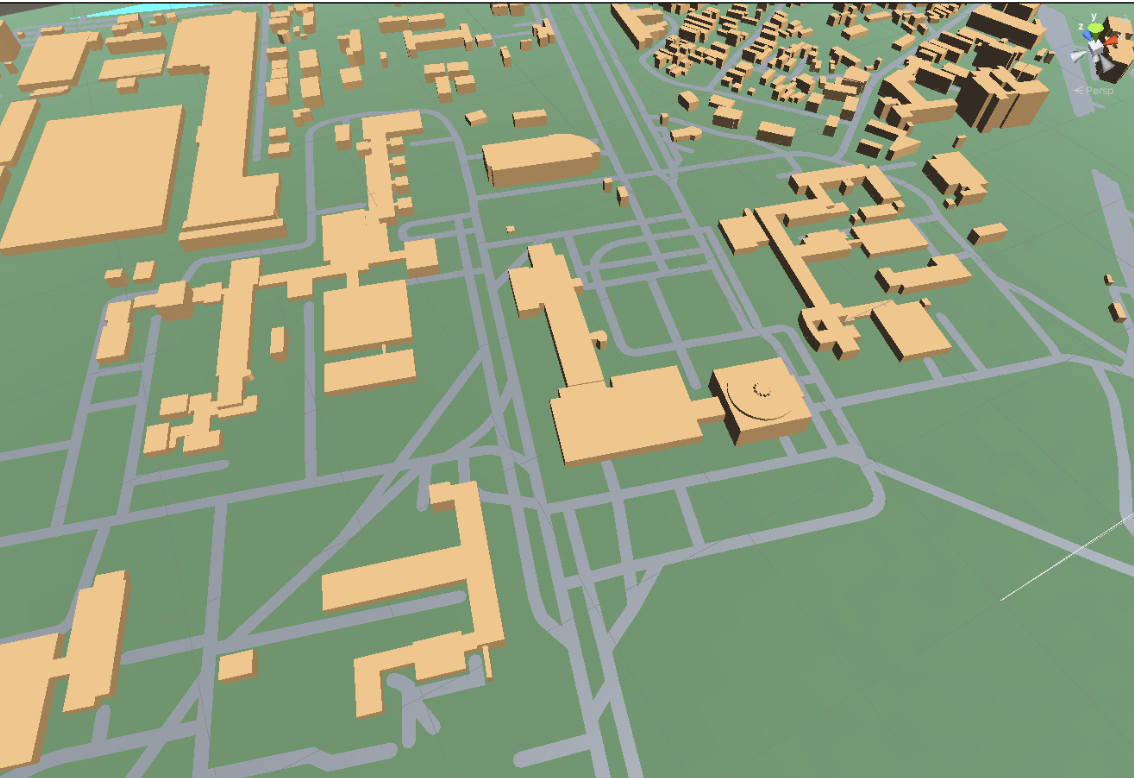
\includegraphics[height=5cm]{figures/demos/maps_sdk_for_unity_buildings.png}
                    \caption{Campus buildings generated using Maps SDK for Unity}
                    \label{3:fig:maps_sdk_for_unity_buildings}
                \end{minipage}
                \hfill
                \begin{minipage}[b]{0.49\textwidth}
                    \captionsetup{justification=centering}
                     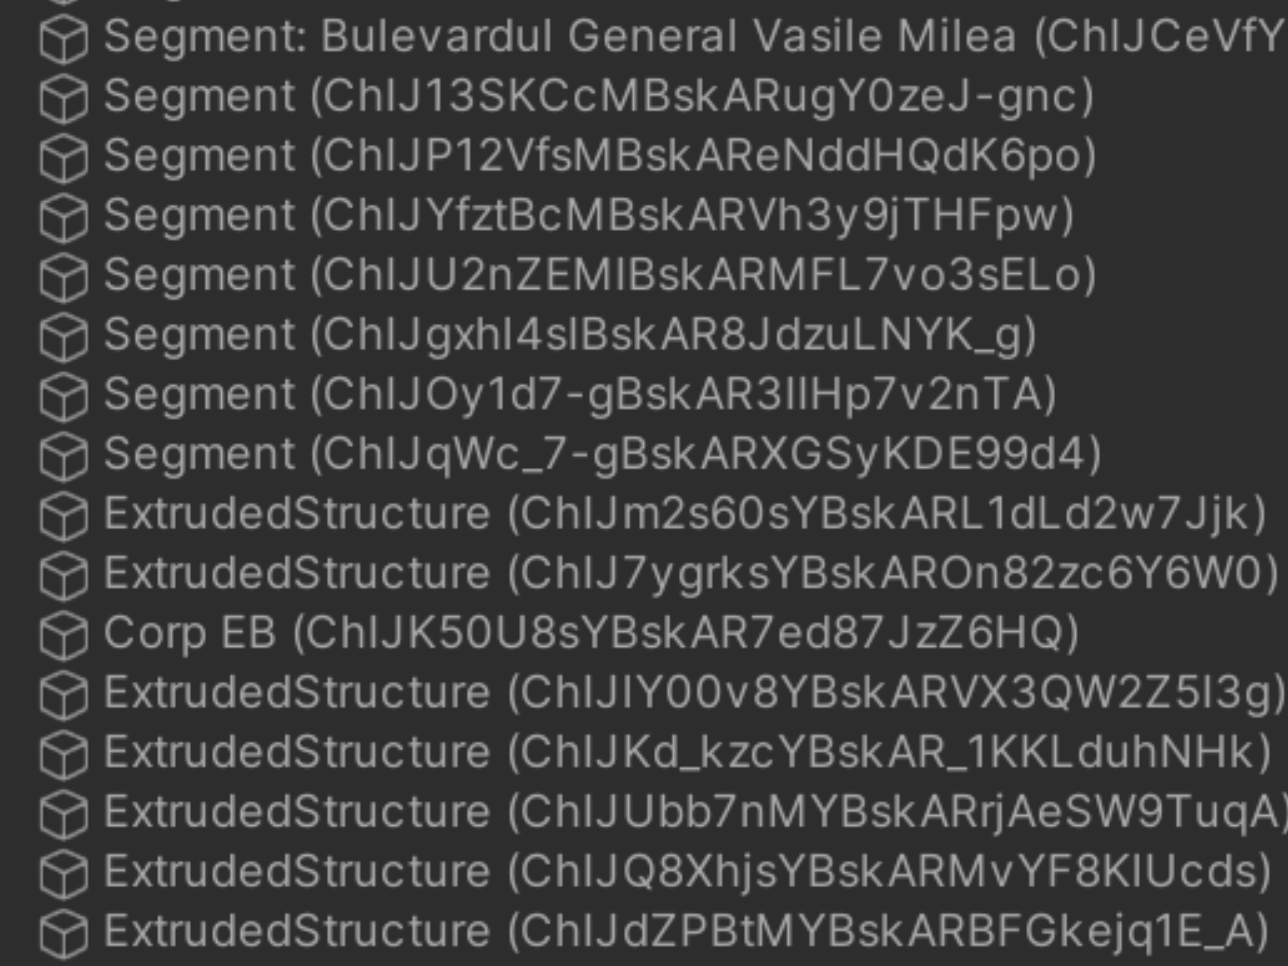
\includegraphics[height=5cm]{figures/demos/maps_sdk_for_unity_gameobjects.png}
                    \caption{Game objects generated by Maps SDK for Unity}
                    \label{3:fig:maps_sdk_for_unity_gameobjects}
                \end{minipage}
            \end{figure}
            
            The metadata associated with these objects includes a \mintinline{text}{Name}, \mintinline{text}{PlaceId} and \mintinline{text}{UsageType} (one of \mintinline{text}{ Unspecified}, \mintinline{text}{ Bar}, \mintinline{text}{ Bank}, \mintinline{text}{Lodging}, \mintinline{text}{ Cafe}, \mintinline{text}{Restaurant}, \mintinline{text}{EventVenue}, \mintinline{text}{TouristDestination}, \mintinline{text}{Shopping} and \mintinline{text}{School}). As not all generated GameObjects map to a place of interest, the default labeling strategy only labels buildings where the name in the metadata is not “ExtrudedStructure” or “ModeledStructure”. However, with this approach and the way our campus buildings are mapped, only three buildings in the entire campus have a label, as shown in figure \ref{3:fig:maps_sdk_for_unity_labels}.
            
            \begin{figure}[ht]
                \centering
                     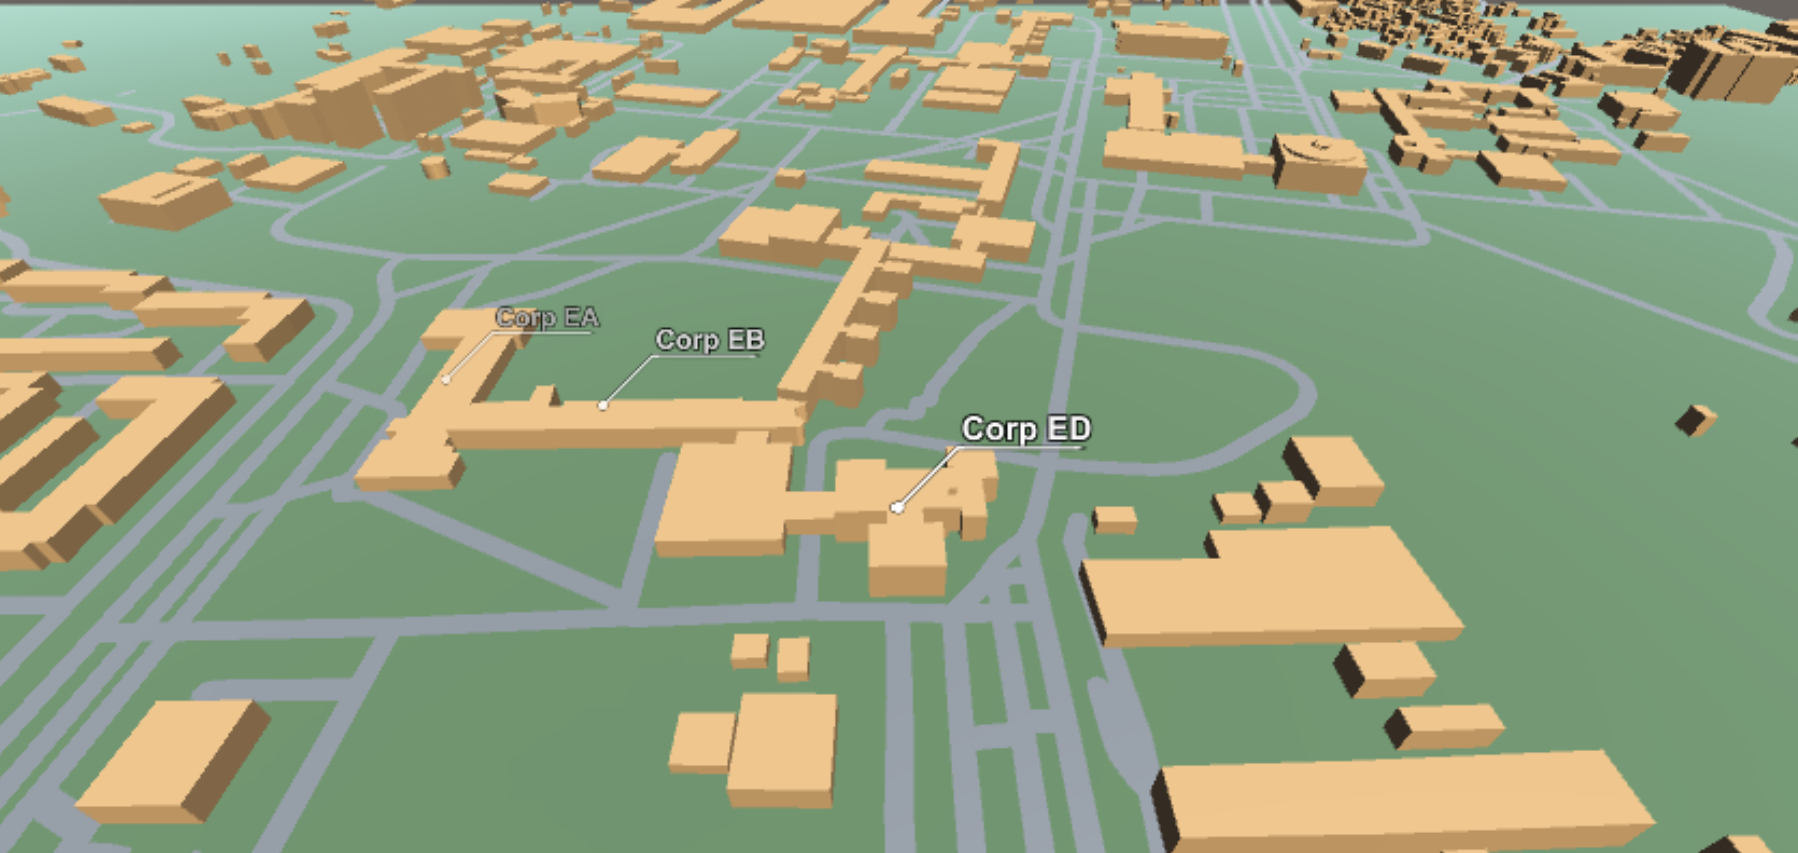
\includegraphics[width=\textwidth]{figures/demos/maps_sdk_for_unity_labels.png}
                    \caption{Campus building labels generated by Maps SDK for Unity}
                    \label{3:fig:maps_sdk_for_unity_labels}
            \end{figure}
            
            Since the data from the Maps API is not sufficient, we could fetch the names of the campus buildings by using the Google Places API\footnote{\url{https://developers.google.com/maps/documentation/places/web-service/overview}}, which offers more information than the basic Maps API. We can do this by making a \mintinline{text}{GET} call and storing the response in a custom serializable class matching the response's structure):
            
            \begin{minted}[breaklines,tabsize=1,frame=single]{csharp}
// Fetch the name of a place via the Places API.
IEnumerator GetPlaceName(GameObject buildingGameObject, string placeId)
{
    string url = "https://maps.googleapis.com/maps/api/place/details/json";
    url += $"?placeid={placeId}&key={mapsService.ApiKey}";
    UnityWebRequest www = UnityWebRequest.Get(url);
    yield return www.SendWebRequest();
 
    if (www.result != UnityWebRequest.Result.Success)
    {
        Debug.Log(www.error);
    }
    else
    {
        var attributes = JsonUtility.FromJson<Place>(www.downloadHandler.text);
        string displayName = attributes.result.name;
 
        Label label = Labeller.NameObject(buildingGameObject, placeId, displayName);
        if (label != null)
        {
            MapsGamingExamplesUtils.PlaceUIMarker(
                buildingGameObject,
                label.transform
            );
        }
    }
}
            \end{minted}
            
            We cannot, however, call this method on every generated GameObject, as not all of them map to a place of interest and a large number of API calls leads the app to consume a lot of resources and freeze. The approach we took next was to try to filter the places we want to fetch more information for, by checking that the \mintinline{text}{UsageType} matches “School”. While this does lead to more buildings being labelled than the previous approach, many are still missing and some are labelled “Bucharest” instead of a useful label, as seen in figure \ref{3:fig:maps_sdk_for_unity_labels_places_api}.
            
            \begin{figure}[ht]
                \centering
                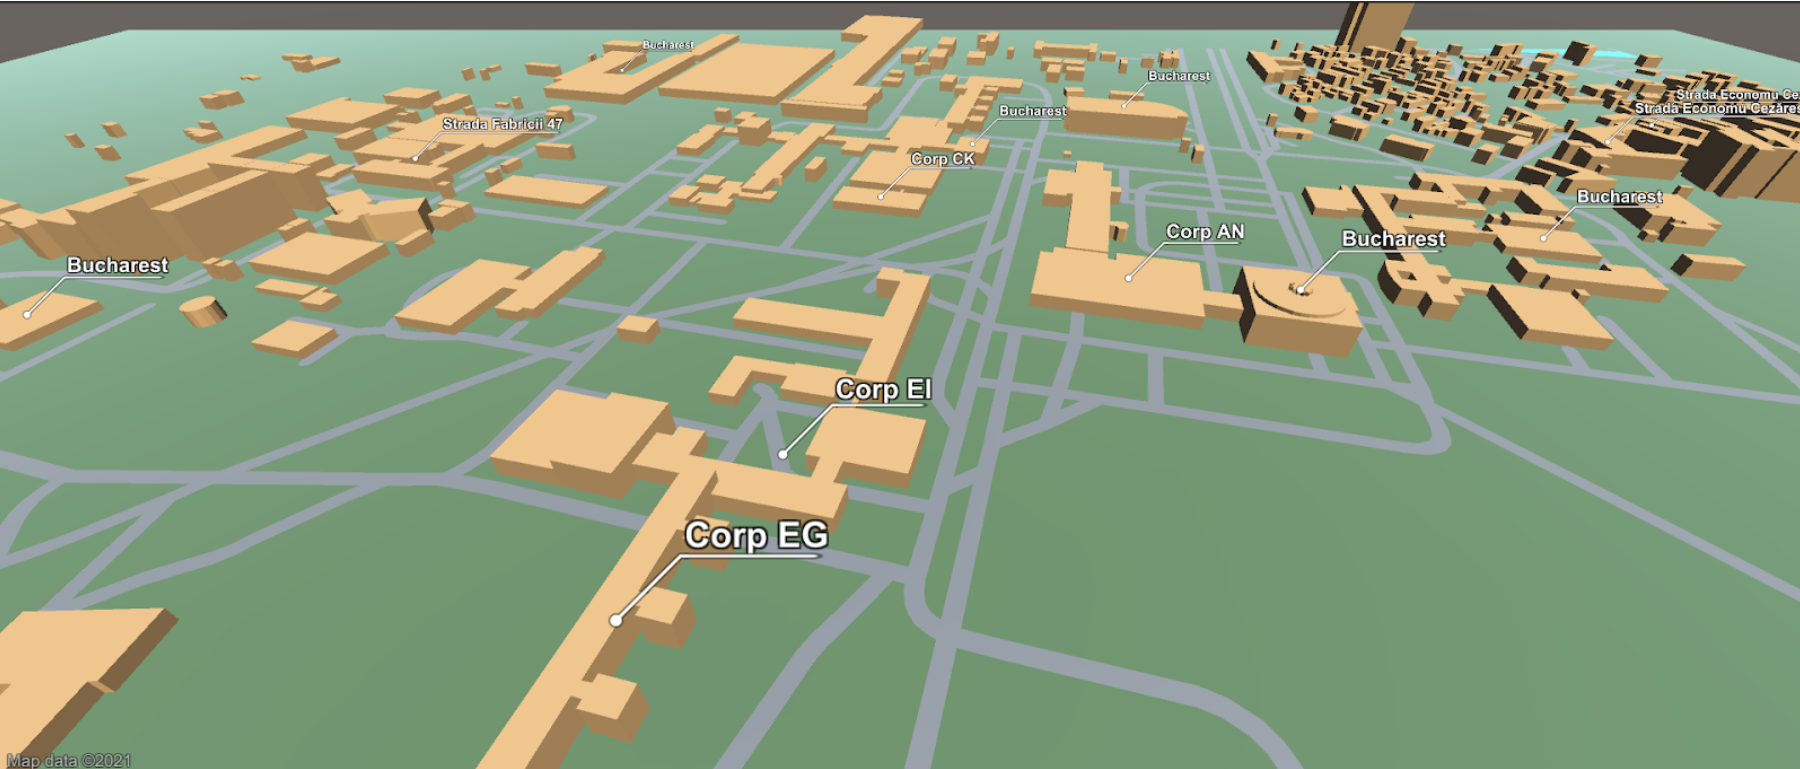
\includegraphics[width=\textwidth]{figures/demos/maps_sdk_for_unity_labels_places_api.png}
                \caption{Campus building labels generated using the Places API}
                \label{3:fig:maps_sdk_for_unity_labels_places_api}
            \end{figure}
            
            We therefore concluded that campus building labels cannot be reliably generated from the Maps/Places APIs. Therefore, the only reasonable solution here is to manually mark the labels of the buildings of interest, alongside their corresponding placeID for the API. We fetch these entries from Firebase so that adding a new building label does not require uploading an app update.
        
        \subsubsection{\gls{flutter} app integration}
        
            \begin{wrapfigure}[25]{l}{0.41\columnwidth}
                \begin{tabular}{@{}cc@{}}
                    \begin{minipage}[b]{0.41\textwidth} 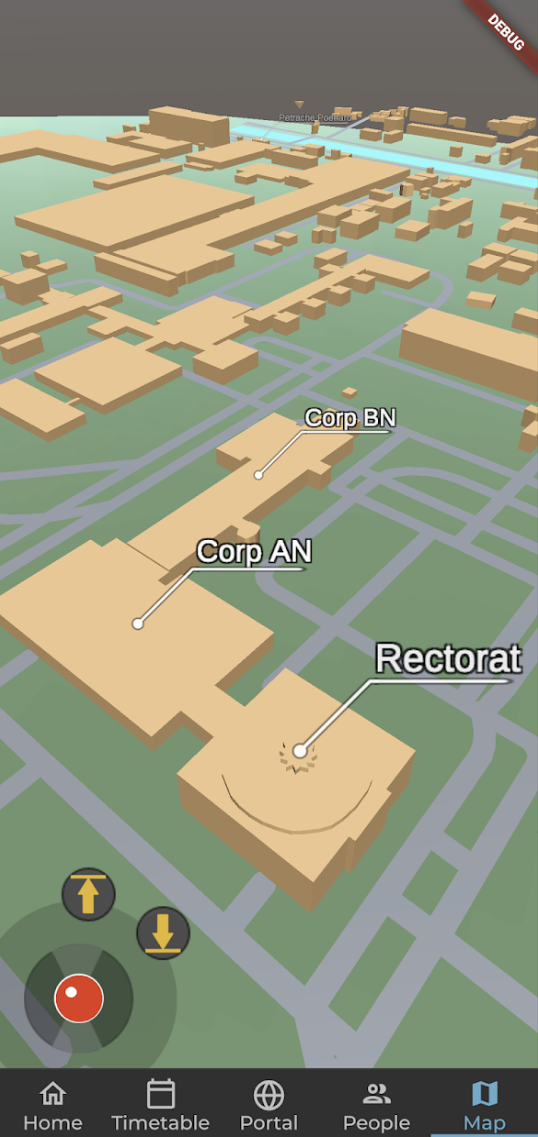
\includegraphics[width=\columnwidth]{figures/demos/maps_sdk_for_unity_flutter.png}
                        \caption{Screenshot of the Map section integrated in \gls{app}}   
                        \label{3:fig:maps_sdk_for_unity_flutter}
                    \end{minipage}
                \end{tabular}
            \end{wrapfigure}
        
            The \mintinline{text}{flutter_unity_widget}\footnote{\url{https://pub.dev/packages/flutter_unity_widget}} allows us to embed Unity into a Flutter app. Since Flutter allows embedding native code and binaries, the widget relies on building the Unity project for each platform (Android and iOS) and linking the result to the two Flutter build targets.
            The package also allows communication between Flutter and Unity through Messages, by using InteropServices\footnote{\url{https://docs.microsoft.com/en-us/dotnet/api/system.runtime.interopservices}} to import native Java (for Android) or Objective-C (for iOS) DLLs into C# to allow calling native methods depending on platform. For Unity->Flutter communication, the messages themselves are serialized as JSON (JObject\footnote{\url{https://www.newtonsoft.com/json/help/html/T_Newtonsoft_Json_Linq_JObject.htm}} in C\#) and sent over as strings which can then be parsed in the onUnityMessage callback in Dart. For Flutter->Unity communication, the package allows us to call exposed GameObject methods directly using \mintinline[breaklines]{csharp}{postJsonMessage(String gameObject, String methodName, Map<String, dynamic> message)}, as long as the gameObject exists and is active in the scene, and the method is exposed through a \mintinline{csharp}{MonoBehaviour} script that uses \mintinline{csharp}{IEventSystemHandler}\footnote{\url{https://docs.unity3d.com/2019.1/Documentation/ScriptReference/EventSystems.IEventSystemHandler.html}}. The message parameter represents a map from method parameter name to its value. We can use this messaging functionality in our app to send a query from Flutter to Unity (e.g. the destination location the user clicked on in an event page, or inputted in a Flutter search bar).
    
    \subsection{Impl. \#2: Indoor (3D) navigation using NavMesh} \label{3:impl2}
    
        Our next approach aims to achieve indoor navigation by drawing a path on a 3D model of the inside of a building of interest.
        
        First, we used Blender\footnote{\url{https://www.blender.org/}} to create a simplified 3D model of a building in our university (EC) based on the floor plan. We then used Unity’s built-in Navigation to bake a NavMesh onto the model, to use for navigation. The NavMesh is visible in blue in figure \ref{3:fig:indoor_navmesh_display}.
        
        \begin{figure}[ht]
            \centering
            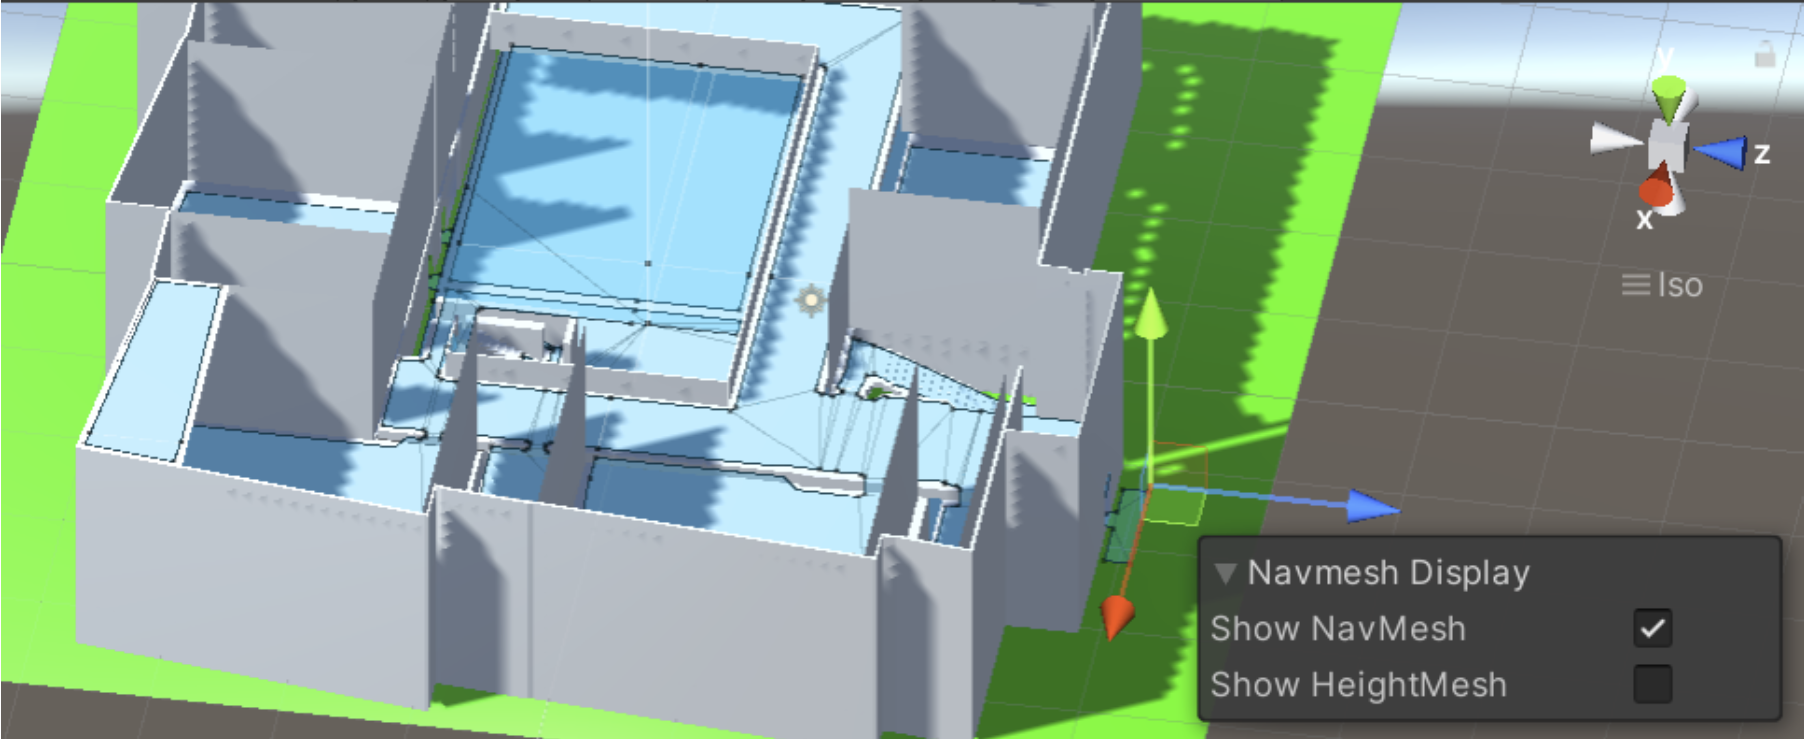
\includegraphics[width=\textwidth]{figures/demos/indoor_navmesh_display.png}
            \caption{NavMesh baked onto the EC building}
            \label{3:fig:indoor_navmesh_display}
        \end{figure}
        
        We then created a \mintinline{text}{NavMeshAgent} representing the user, and added support for clicking on a spot on the mesh in order to mark the destination. Once a destination is chosen, a path is drawn on the mesh between the agent and the destination, representing the recommended navigation route (fig. \ref{3:fig:indoor_navmesh_path}) .
        
        \begin{figure}[ht]
            \centering
            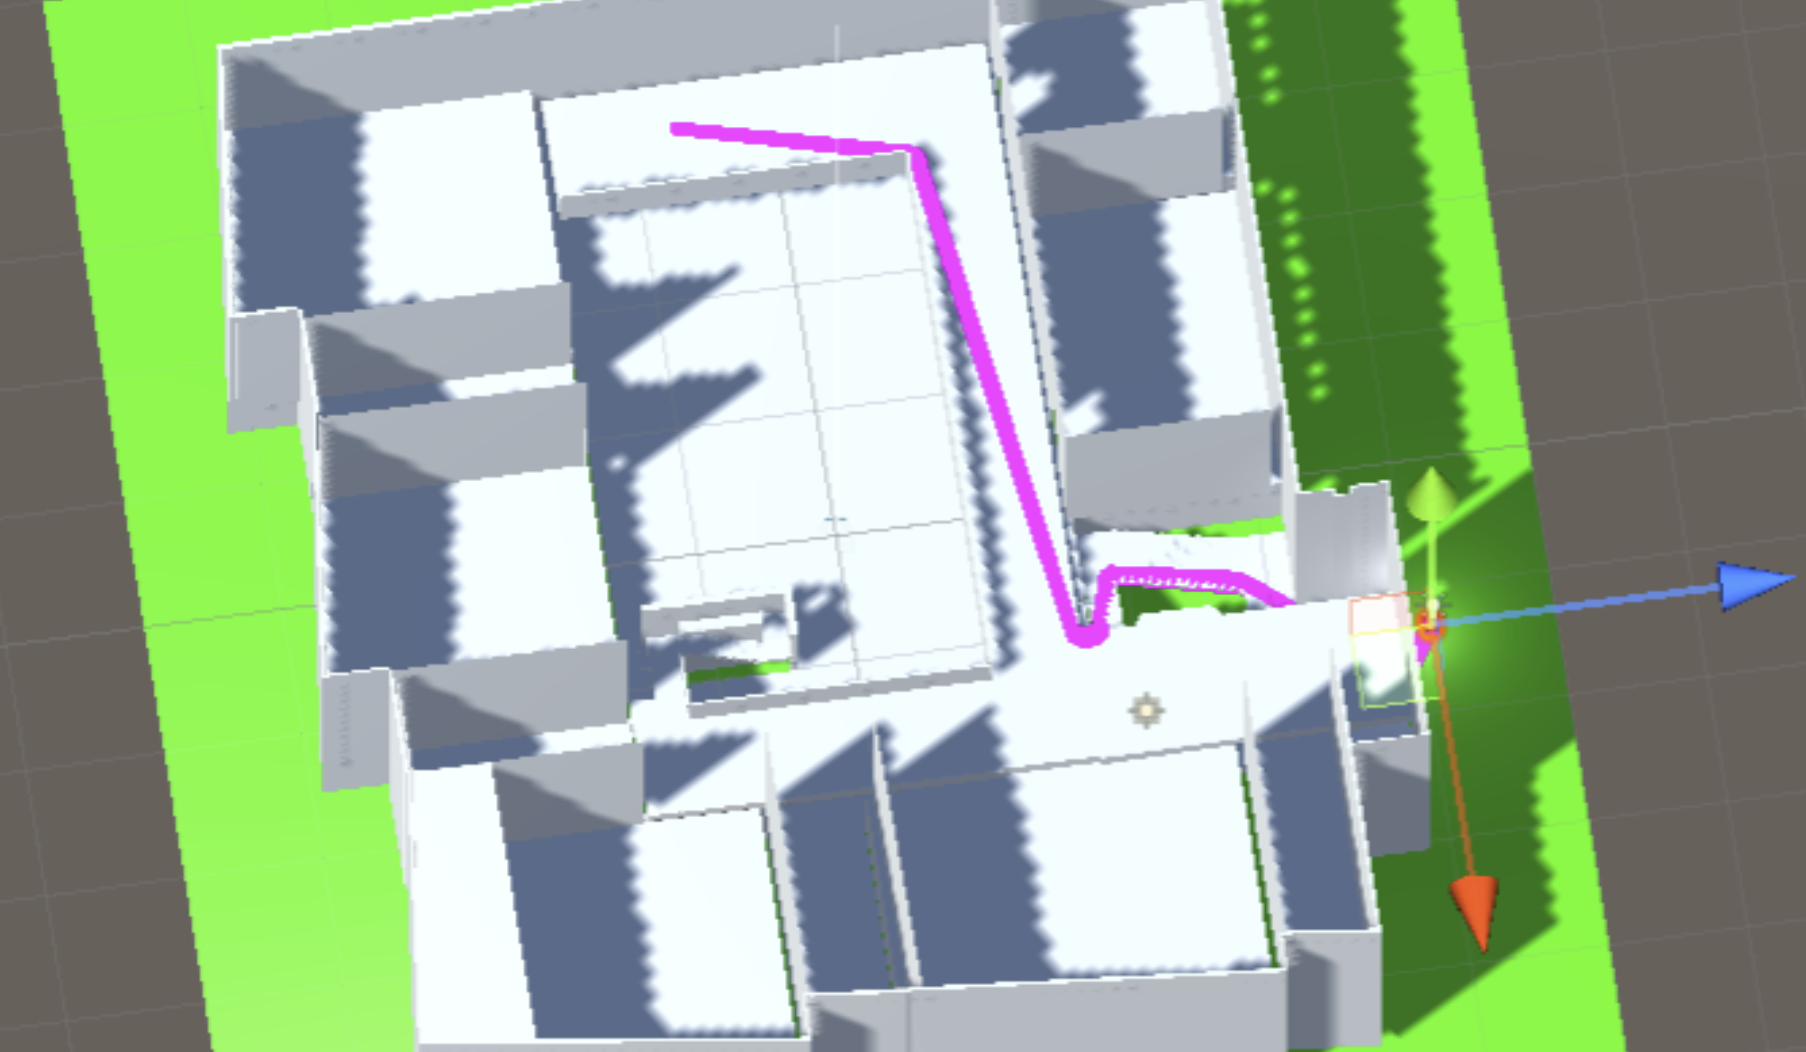
\includegraphics[width=\textwidth]{figures/demos/indoor_navmesh_path.png}
            \caption{Navigation path drawn using NavMesh}
            \label{3:fig:indoor_navmesh_path}
        \end{figure}
        
        
        \begin{wrapfigure}[17]{l}{0.35\columnwidth}
            \begin{tabular}{@{}cc@{}}
                \begin{minipage}[b]{0.35\textwidth} 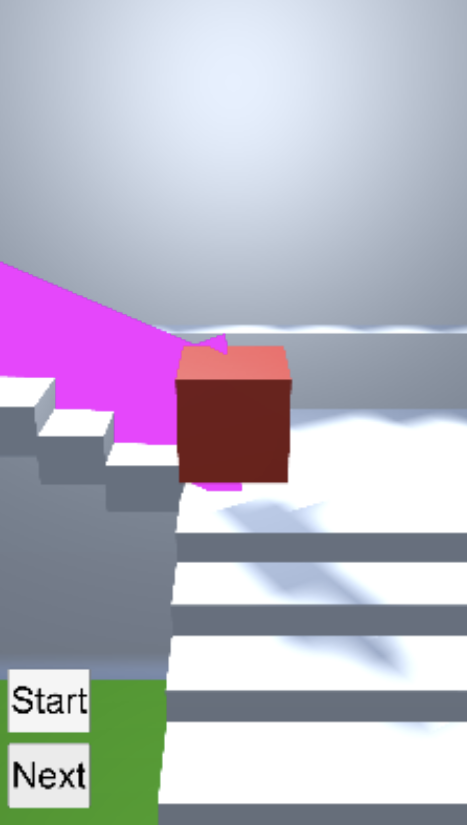
\includegraphics[width=\columnwidth]{figures/demos/indoor_navmesh_3p.png}
                    \caption{Third-person navigation view}   
                    \label{3:fig:indoor_navmesh_3p}
                \end{minipage}
            \end{tabular}
        \end{wrapfigure}
        
        In the 3rd person player view, for the proof of concept we added two buttons - a “Start” button which triggers drawing the navigation path to the destination, and a “Next” button which moves the agent to the next “turn” (node) in the path. As such, the user can manually select a location as the destination, as well as their current location, and be guided step by step through each segment of the path.
        
        As an alternative to the low-fidelity 3D model built based on the floor plan, we also tried to use a model of the building from the 3DUPB archive (fig. \ref{3:fig:ed_model}). However, these models are designed to be as accurate as possible, including the furniture and decorative elements in the buildings. This lead to a significantly more complex NavMesh and much higher latency, making it unsuitable for a mobile application. These models could, of course, be simplified, but we have found that using a simple model made from scratch is the more scalable approach.
            
        \begin{figure}[!ht]
            \centering
            \begin{minipage}[b]{\textwidth}
                \captionsetup{justification=centering}
                 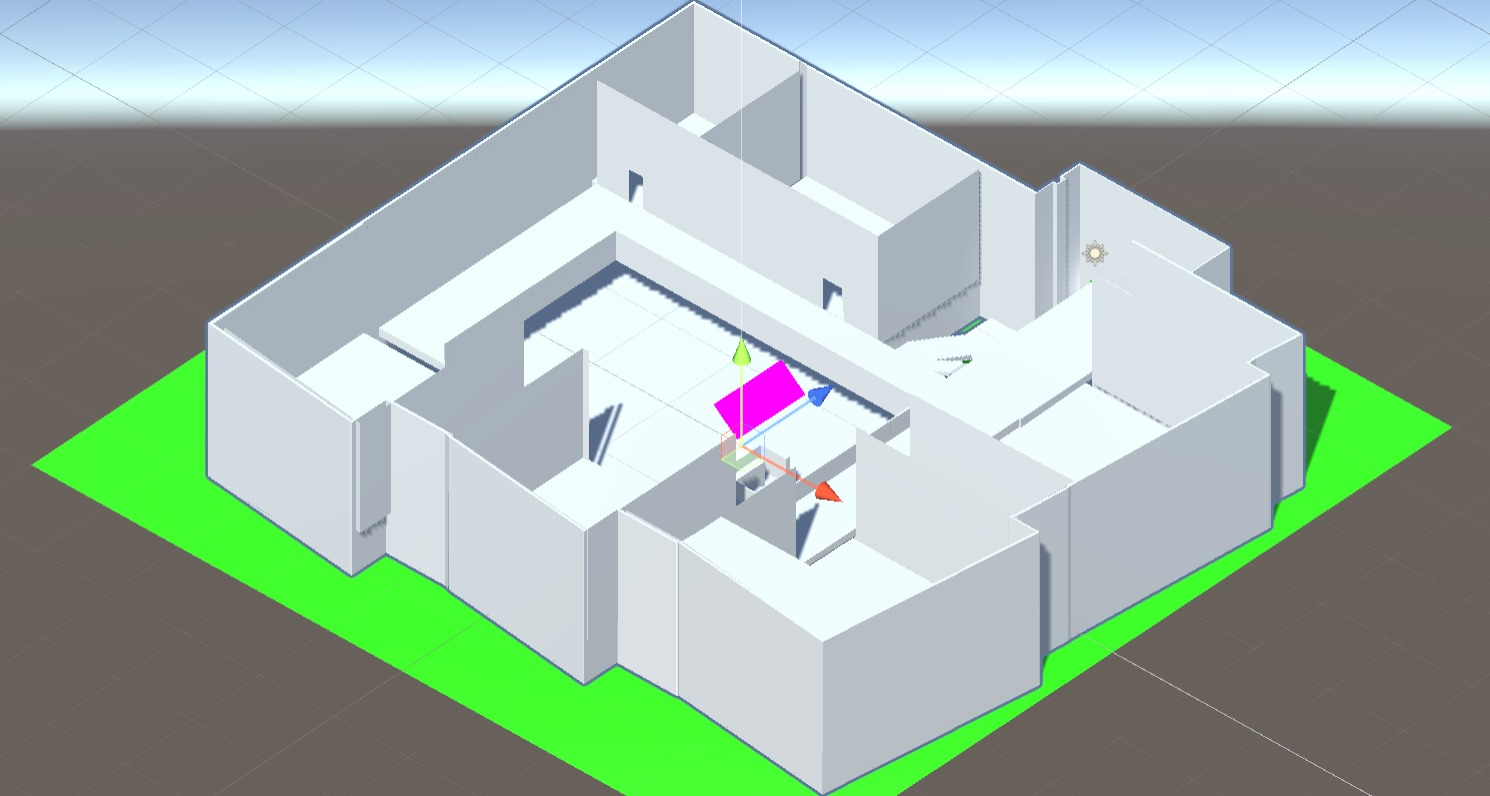
\includegraphics[width=0.49\textwidth]{figures/demos/ec_model_simple.jpeg}
                 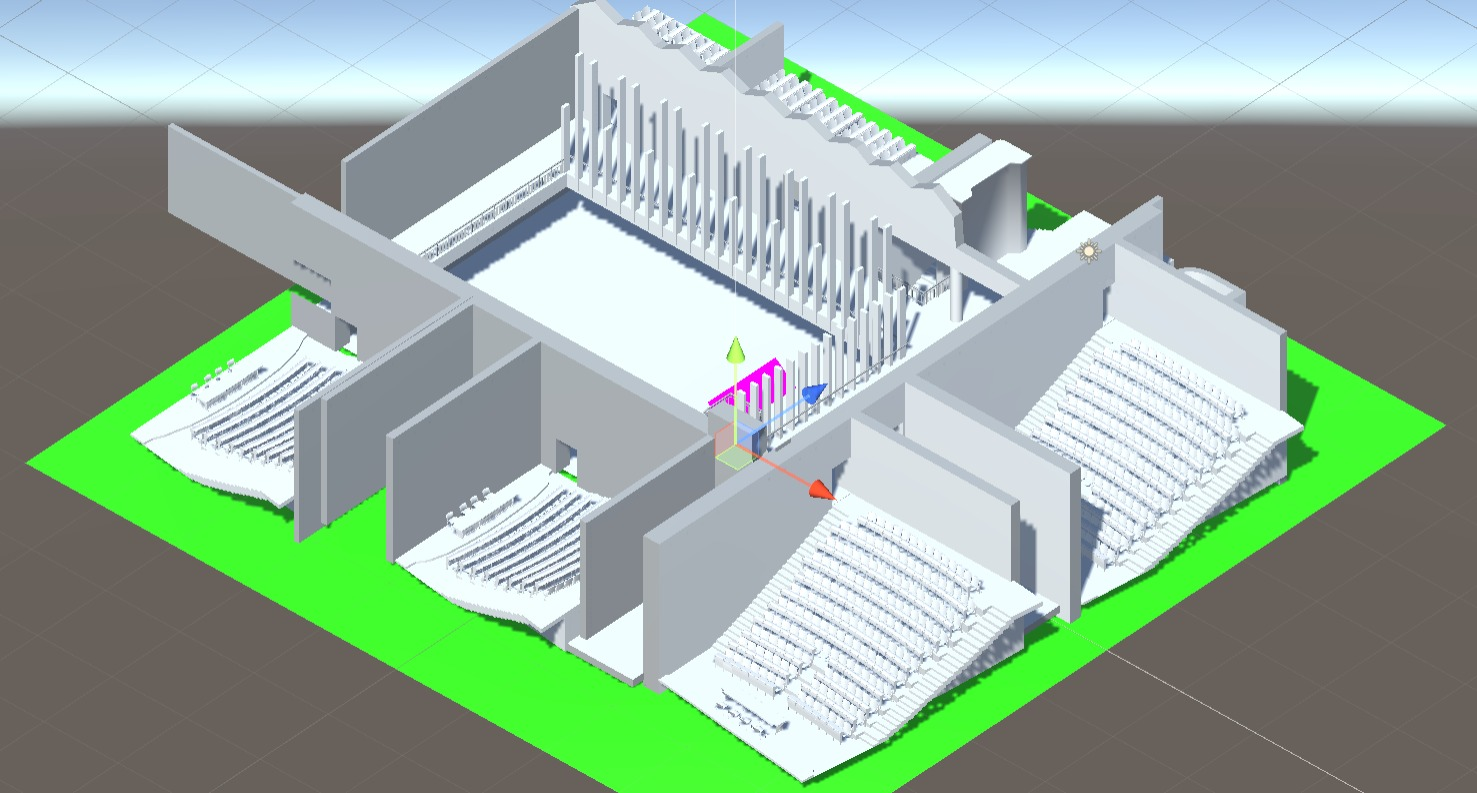
\includegraphics[width=0.49\textwidth]{figures/demos/ec_model_3dupb.jpeg}
                \caption{Floorplan-based low fidelity model (left) vs. 3DUPB high-detail model (right)}
                \label{3:fig:ed_model}
            \end{minipage}
        \end{figure}
    
    \subsection{Impl. \#3: Outdoor (3D) navigation with MapsModelsImporter} \label{3:impl3}
    
        For our third implementation, we test out a different approach to outdoor navigation using a 3D map imported from Google Maps. For this, we use MapsModelsImporter\footnote{\url{https://github.com/eliemichel/MapsModelsImporter}}, a Blender add-on for importing 3D models from Google Maps. As such, we imported multiple meshes corresponding to the campus map, overlapped and merged them together in Blender (fig. \ref{3:fig:mapsmodelsimporter_blender}).
        
        \begin{figure}[ht]
            \centering
            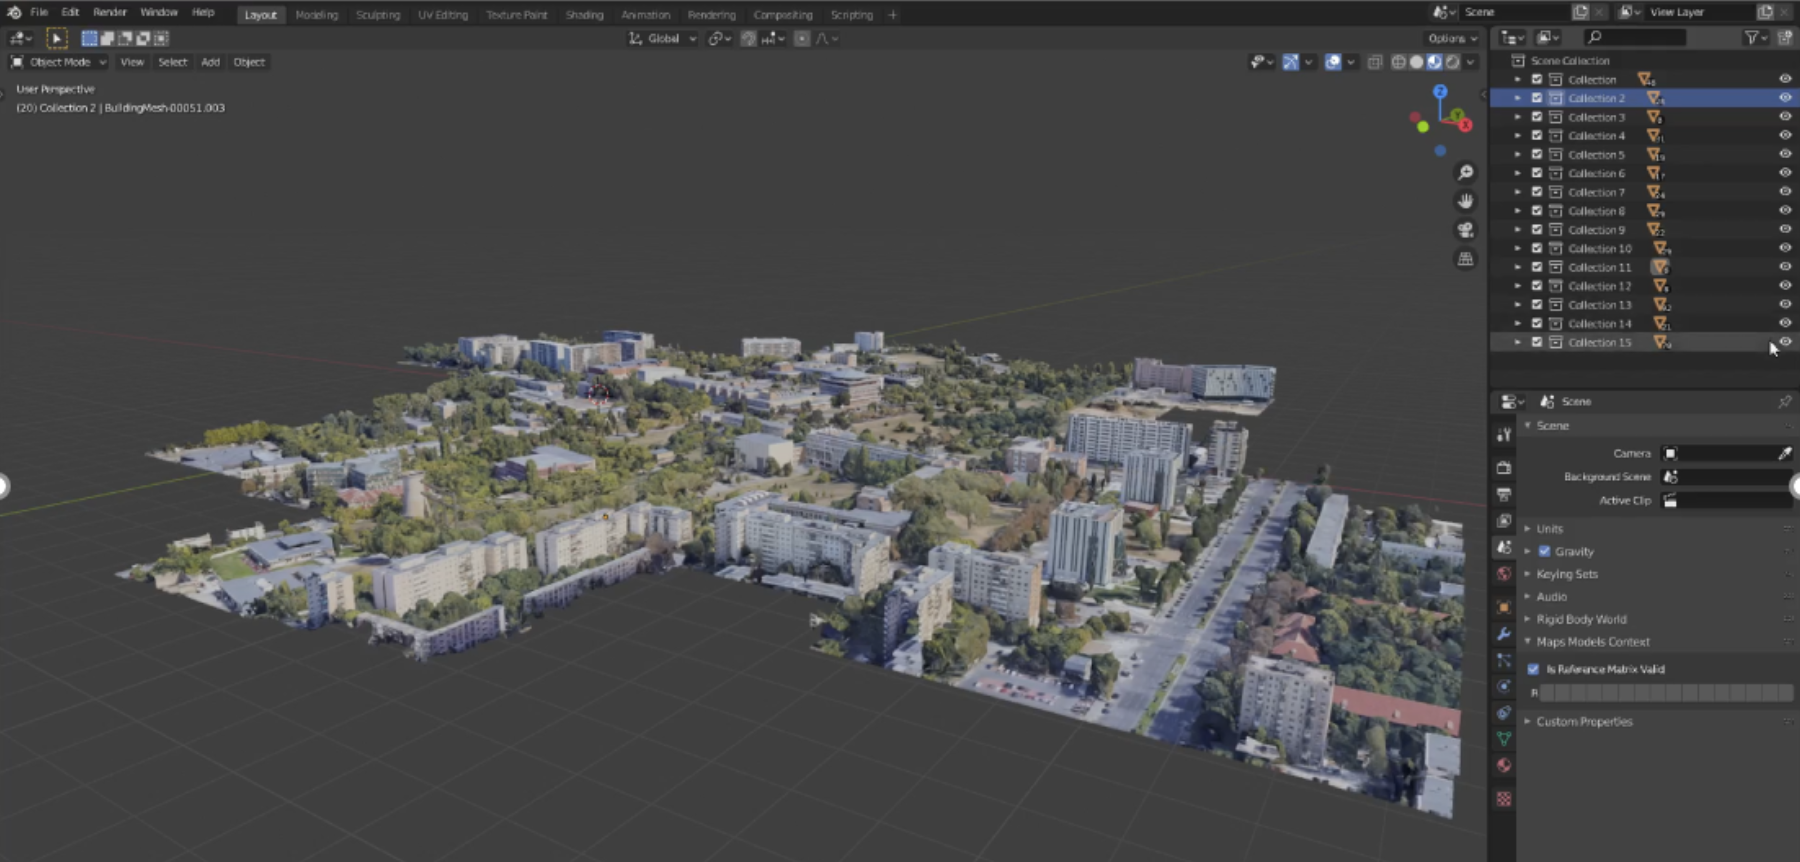
\includegraphics[width=\textwidth]{figures/demos/mapsmodelsimporter_blender.png}
            \caption{Map model imported in Blender using MapsModelsImporter}
            \label{3:fig:mapsmodelsimporter_blender}
        \end{figure}
        
        \begin{wrapfigure}[16]{l}{0pt}
            \begin{tabular}{@{}cc@{}}
                \begin{minipage}[b]{0.35\textwidth} \           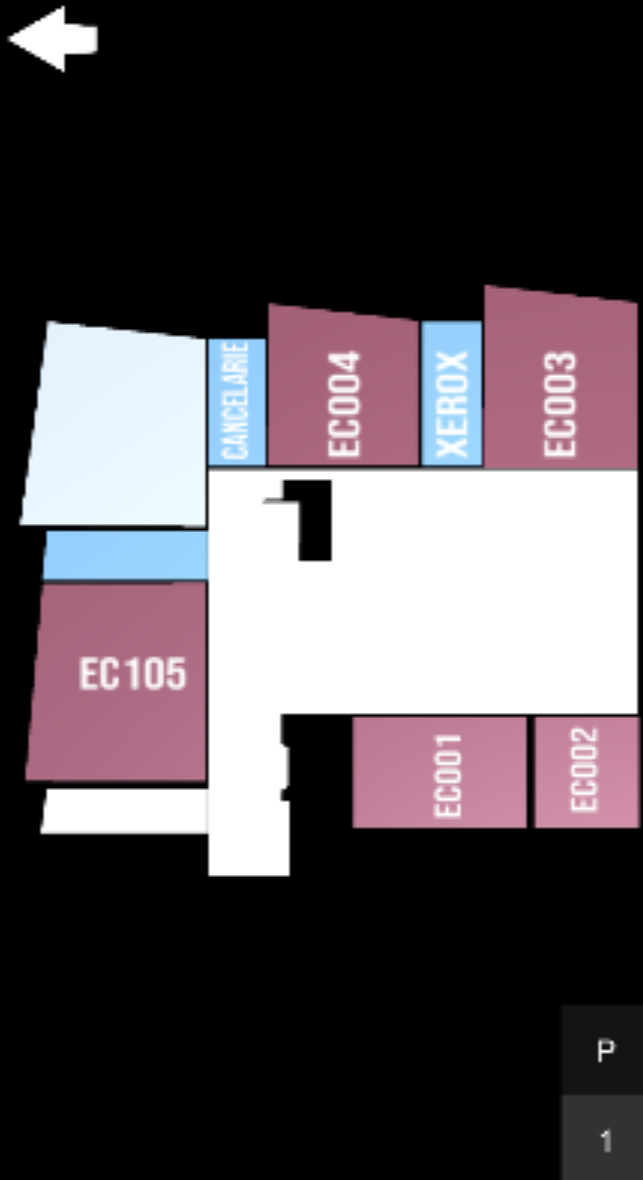
\includegraphics[width=\columnwidth]{figures/demos/unity_floorplan.png}
                    \captionsetup{justification=centering}
                    \caption{Floorplan Unity module}   
                    \label{3:fig:unity_floorplan}
                \end{minipage}
            \end{tabular}
        \end{wrapfigure}
        
        The floor plan GameObject was created by drawing an SVG and importing it into Blender as a mesh. This allows us to have separate objects for each different room in Unity, in order to define on-click behaviours using ray casting.
        
        Each room has a unique identifier, so we can also fetch additional information about it from Firebase (such as type, room capacity, building & floor it belongs to etc.).
        
        The Firebase integration allows us to easily update room information remotely, without requiring an app update. However, the same cannot be said for the actual campus maps - these are imported as Unity objects, and therefore included in the app executable. Fortunately, we don't expect the maps to change very often.
        
        ~
        
        ~
        
        Furthermore, for this demo we also use standard GPS (location services) to place the agent (user) on the map:
        
        \begin{minted}[breaklines,tabsize=1,frame=single]{csharp}
if (Input.location.status == LocationServiceStatus.Running)
{
    // Access granted to GPS values & it has been initialised
    float x = latToX(Input.location.lastData.latitude);
    float z = lonToZ(Input.location.lastData.longitude);
    player.transform.position = new Vector3(x, 0.8f, z);
}
        \end{minted}
        
        Finally, we again use Unity’s NavMesh to create paths from the user’s GPS location to a point of interest. We currently use the auto-generated NavMesh (fig. \ref{3:fig:mapsmodelsimporter_path}), but it can be improved by manually drawing the mesh over the areas representing a walkable paths (alleys, roads in the campus).
        
        \begin{figure}[ht]
            \centering
            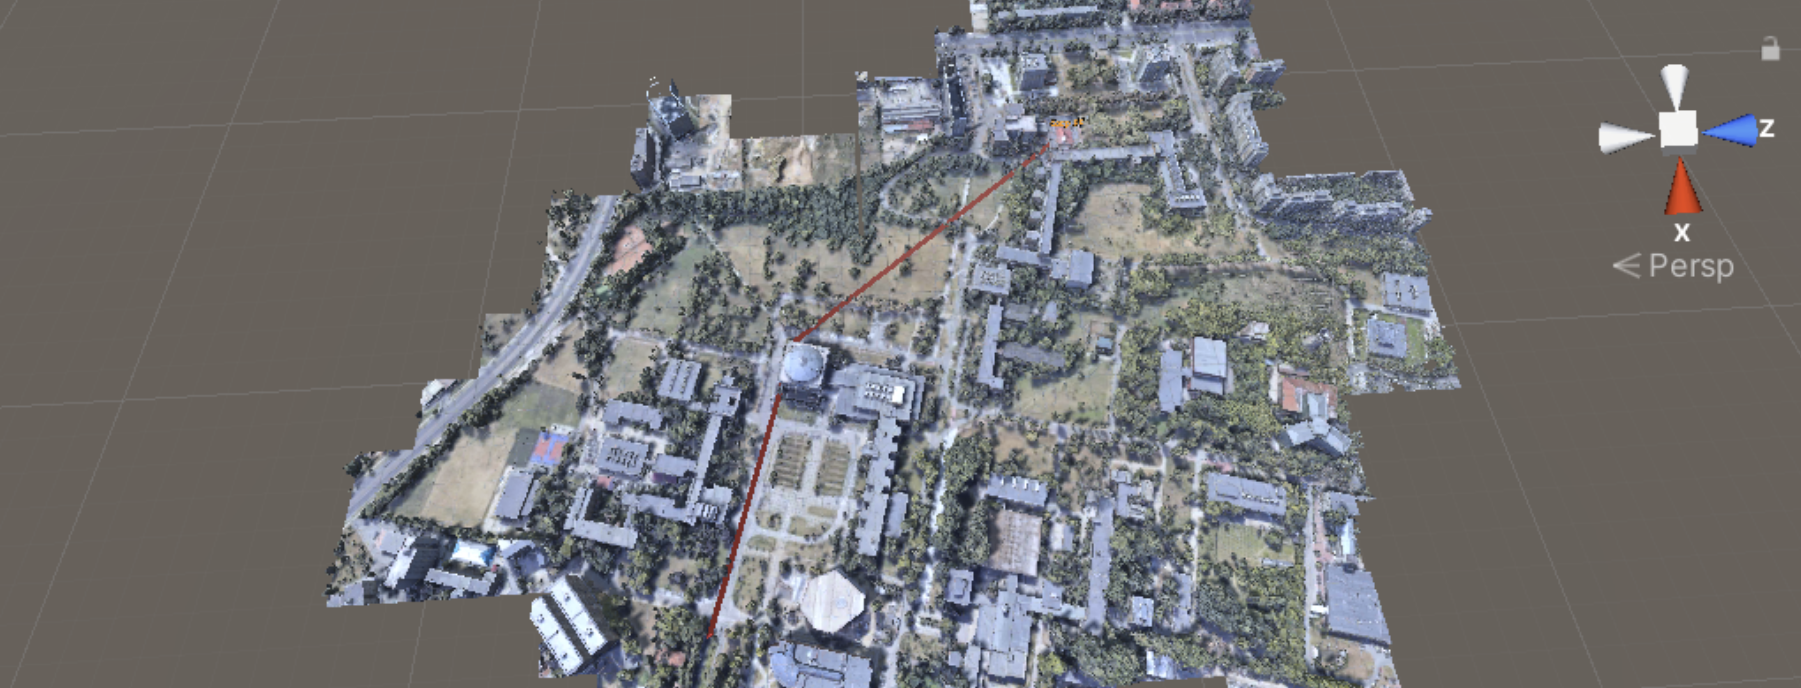
\includegraphics[width=\textwidth]{figures/demos/mapsmodelsimporter_path.png}
            \caption{Path drawn on MapsModelsImporter map}
            \label{3:fig:mapsmodelsimporter_path}
        \end{figure}
    
    \subsection{Impl. \#4: AR-powered indoor navigation}\label{3:impl4}
    
        For our final indoor navigation implementation, we explore AR navigation using \acrshort{slam}. This approach is based on an article by CRAFTWORKZ's Jan Hardy\cite{hardy2020arnavigation} and an article by Roberto Lopez Mendez from Arm Community\cite{mendez2018arnavigation}.
        
        Due to not having access to the campus while testing, we tested the initial proof of concept at home, using a floor plan created by a robot vacuum. However, this solution is not highly dependent on the location, and can easily be adjusted with any map, as long as it is to scale.
        
        We started by creating a plane with the floorplan in Unity. In order for the tracking to work correctly, we also needed to make sure that the scale of the map in Unity matches real life (1 meter in real life = 1 distance unit in Unity). If this scale is not correct, the position of the user on the map will seem to be moving too slowly or too quickly.
        
        We then used the Google ARCore Extenssions for AR Foundation\footnote{\url{https://github.com/google-ar/arcore-unity-extensions}} package to integrate AR functionality, and created a script that translates real life movement to the movement of a sphere, chosen to represent the user's location. This allows us to move the sphere on the map as the user moves with their AR camera, using \acrshort{slam}.
        
        Once the sphere can be moved according to the user's movement, we need to also make sure that the starting point corresponds to the user's starting point. GPS location is not accurate enough, so we chose to add some anchor points on the map that the user can start navigating from. These points have an ID associated with them, and this ID can be fetched by scanning a QR code at that specific location (fig. \ref{3:fig:qr_scanning}). For the QR scanning functionality, we use the ZXing.Net library\footnote{\url{https://github.com/micjahn/ZXing.Net}}.
        
        Finally, for the actual navigation, we again use NavMesh to map the walkable area on the map and draw a path to the destination. We show this path on the 2D minimap in the app, in addition to an arrow pointing to the direction where the user has to go (fig. \ref{3:fig:ar_navigation}).
        
        \begin{figure}[!ht]
            \centering
            \begin{minipage}[b]{0.4\textwidth}
                \captionsetup{justification=centering}
                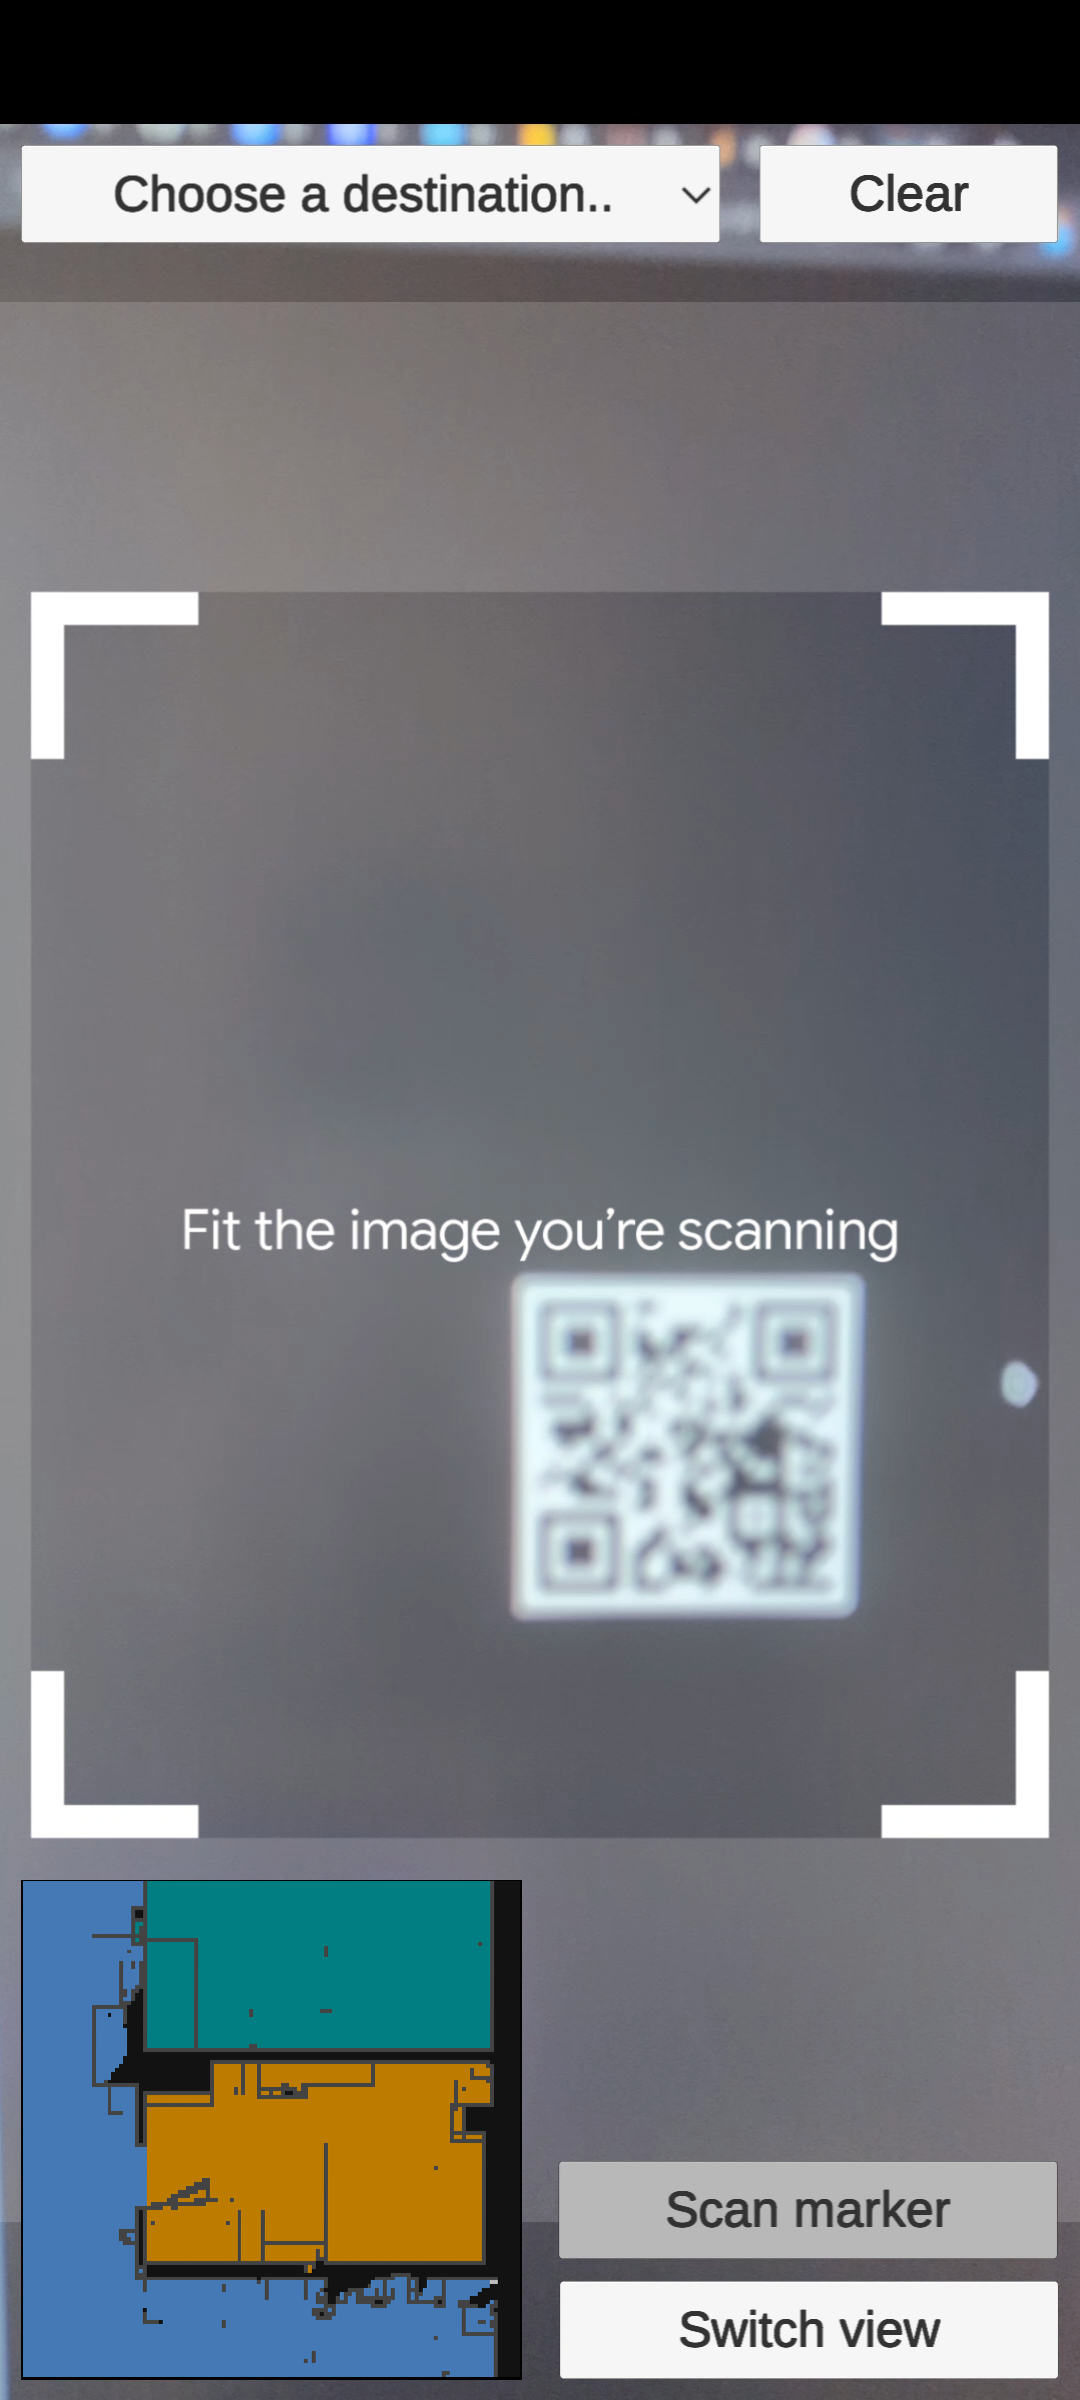
\includegraphics[width=\textwidth]{figures/demos/qr_scanning.png}
                \caption{QR scanning for the initial positioning}
                \label{3:fig:qr_scanning}
            \end{minipage}
            \hfill
            \begin{minipage}[b]{0.4\textwidth}
                \captionsetup{justification=centering}
                 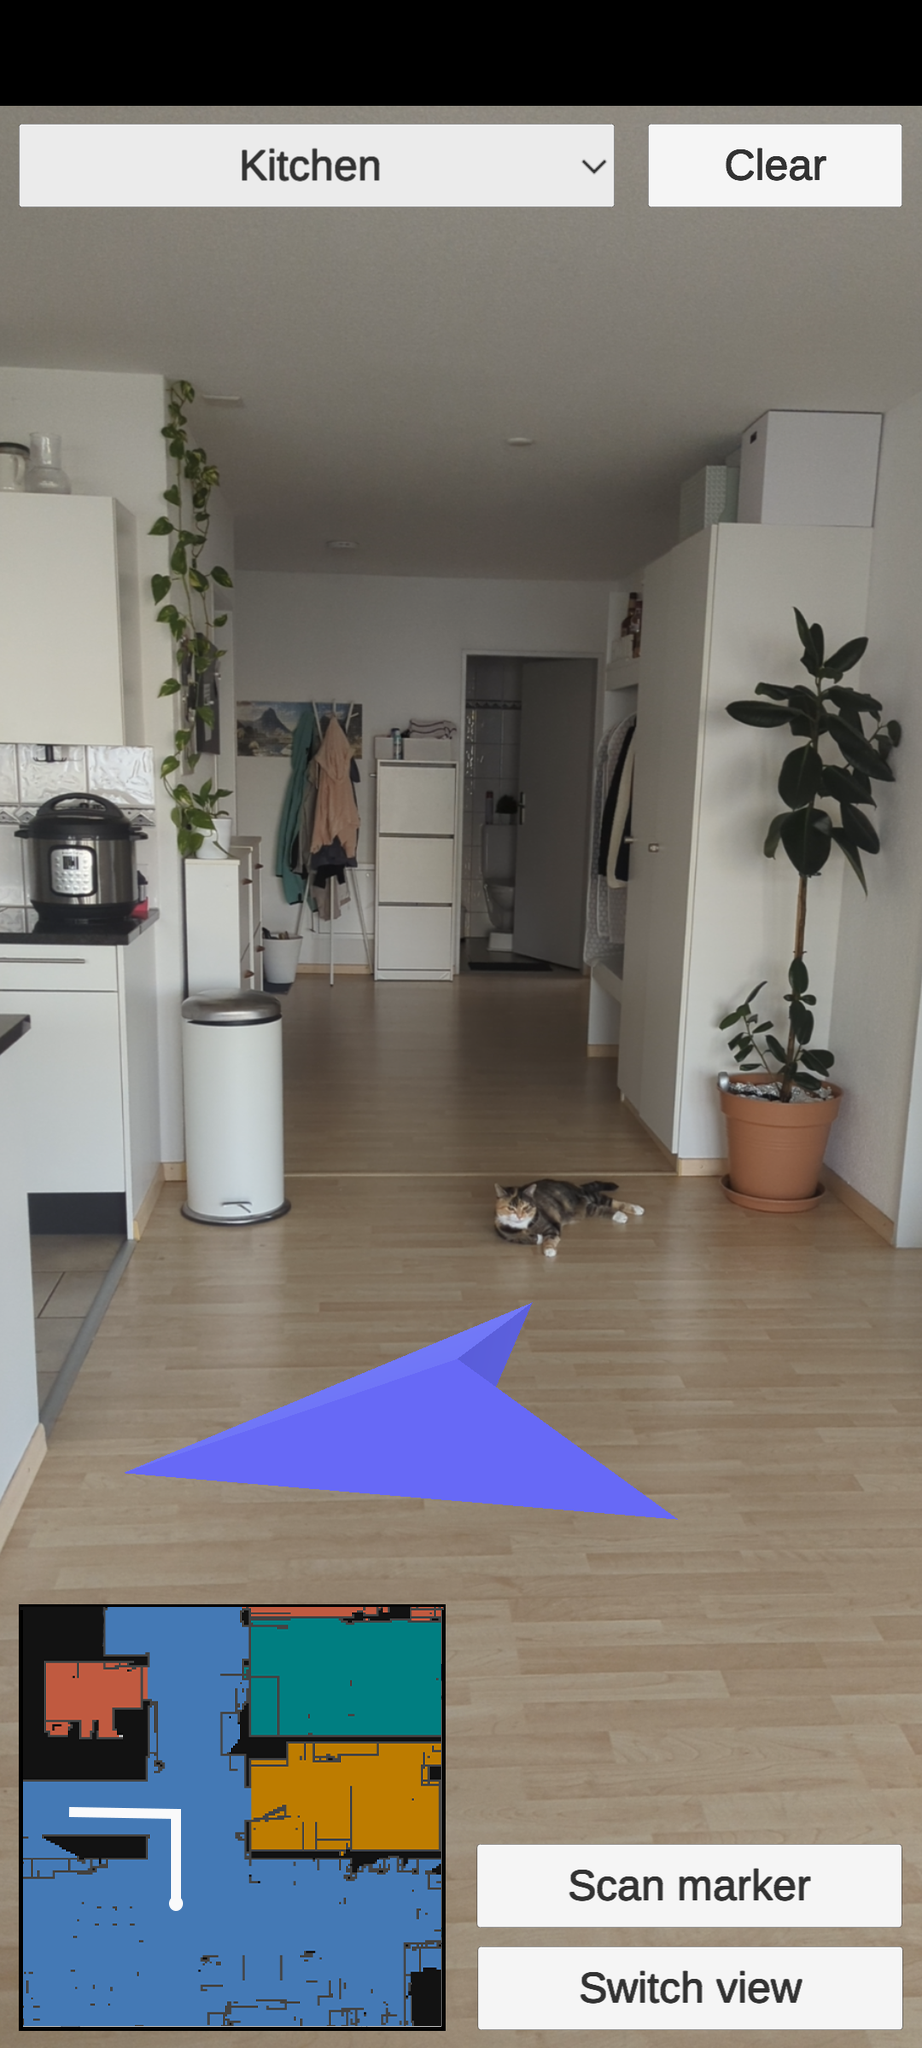
\includegraphics[width=\textwidth]{figures/demos/ar_navigation.png}
                \caption{AR indoor navigation experience}
                \label{3:fig:ar_navigation}
            \end{minipage}
        \end{figure}
    
    \subsection{Bonus module: 360° image viewer} \label{3:360}
    
        As an additional feature to navigation, we created a module for viewing 360° images of various points of interest in the campus. We reached out to the photographer who created the UPB Virtual Tour\footnote{\url{http://turvirtual.upb.ro/}}, and he gave us access to all 360° images in the university's virtual tour collection. These images are fetched directly from our cloud storage, so as not to unnecessarily increase the app size. Users Would be able to tap certain points of interest on the map and view the relevant 360° photo taken from that point.
        
        In terms of implementation, a spherical image viewer was implemented in Unity using the Skybox (fig. \ref{3:fig:360_image_viewer}). Touch controls were also added, to allow the user to pan and zoom.
        
        \begin{figure}[ht]
            \centering
            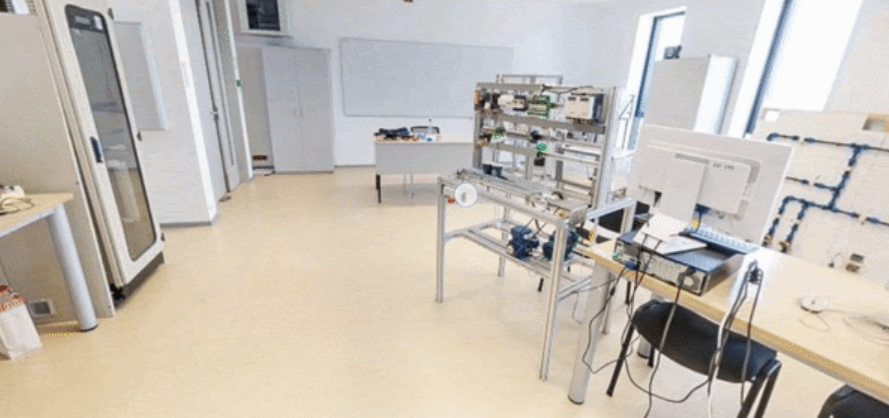
\includegraphics[width=\textwidth]{figures/demos/360_image_viewer.png}
            \caption{360° image viewer}
            \label{3:fig:360_image_viewer}
        \end{figure}
    
\section{Comparison}

    Table \ref{3:tab:impl_comparison} illustrates the variables (explained in section \ref{3:alternatives_considered}) selected for each of the four proofs of concept described in the previous section.

    \begin{table}[th]\small\linespread{1}
        \caption{Implementation comparison}
        \label{3:tab:impl_comparison}
        \centering
        \resizebox{\textwidth}{!}{
        \begin{tabular}{|L{2.45cm}|C{2.55cm}|C{2.55cm}|C{2.55cm}|C{2.55cm}|}
            \cline{2-5}
            \multicolumn{1}{c|}{} & \textbf{Impl. \#1} & \textbf{Impl. \#2} & \textbf{Impl. \#3} & \textbf{Impl. \#4} \\ \hline
            \textbf{Goal} & outdoor navigation & indoor navigation & outdoor navigation & indoor navigation  \\
            \hline
            \textbf{Technologies, tools and APIs} & \gls{unity}, \gls{flutter}, Google Maps SDK for Unity, Firebase & \gls{unity}, Blender, Firebase & \gls{unity}, Blender, MapsModelsImporter & \gls{unity}, ZXing, ARCore, Firebase, Photoshop \\
            \hline
            \textbf{Map representation} & 3D, low detail & 3D, low \& high detail & 3D, high detail & 2D  \\
            \hline
            \textbf{Integrations} & directly as a page \gls{app} & - & - & using UPB Campus room data  \\
            \hline
            \textbf{Source of truth} & Google Maps (dynamic) & fixed building model & Google Maps (fixed) &  fixed floor plan \\
            \hline
            \textbf{Pathfinding} & A* & NavMesh & NavMesh &  NavMesh \\
            \hline
            \textbf{Initial positioning} & user input & user input & GPS &  QR code \\
            \hline
            \textbf{Movement tracking} & user input & user input & GPS &  AR with SLAM \\
            \hline
        \end{tabular}
        }
    \end{table}
        
    A comparison of these approaches in terms of user experience can be found in section \ref{4:demos} in the following chapter.
    